\section{Process discovery through Grammar Inference} \label{grammar}
One of the most relevant to my research work done by Cook \& Wolf in \cite{citeulike:328044}. Authors developed techniques which they called \textit{``process discovery''}: they designed a framework which collects a software process data from ongoing process and generates a set of recurring patterns of behavior characterizing observed process. Under this work they augmented two methods of \textit{grammar inference} from previous work: neural network based and purely algorithmic method as well as developed their own Markovian method. The grammar inference can be defined as the process of infering a language grammar from the given set (sample) of sentences in the language. Once the grammar is inferred it could be converted into the (N)DFA which visualizes the observed phenomena. 

\begin{figure}[tbp]
   \centering
   \includegraphics[height=70mm]{inference.eps}
   \caption{Process discovery through the grammar inference: panel a) a sample event stream (simple process involving three types of events: Edit, Review, and Checkin); and FNA results obtained by applying three methods of process discovery from Cook \& Wolf \cite{citeulike:328044}.}
   \label{fig:inference}
\end{figure}

The first method, neural network based grammar inference method RNet, adopted by authors defines a recurrent neural network architechture which characterizes current system state looking on the past behavior. Once the neural net is trained, authors extract the FSM by presenting different strings to the net and extracting the hidden neurons activity through observations. By the nature of Neural Net, the closely related activation patterns clustered into the same state. By noting the current pattern, the input token, and the next activation pattern transitions are recorded and compiled into inferred FSM later.

The second approach taken, a purely algorithmic KTail method, augmented by authors from Biermann \& Feldman \cite{citeulike:5120603}. The idea is that a state is defined by what future behaviors can
occur from it. The \textit{future} is defned as the set of next $k$ tokens. Obviously, two or more strings can share a common prefix and then diverge from each other providing features for building a corresponding FSM.

The Markov based method developed by authros is taking in account past and future system behavior in order to guess the current system state. Assuming that a finite number of states can defined the process, and that the probability of the next state is based only on the current state (Markov property) authors build a $n^{th}$-order Markov model using the first and second order probabilities only. Once built, the probability table corresponding to the markov model converted into FSM which further reduced basing on the user specified cut-off threshold for probabilities.

Authors implemented all discussed algorithms in a software tool called DaGama as a plugin for larger software system Balboa \cite{citeulike:5120757}. 

Overall, while having some issues with the complexity of produced output and noise handling, authors proved applicability of implemented algorithms to the real-world process data by demonstrating an abstraction of the actual process executions and capturing important properties of the process behavior. Major backdraw of the approach as stated by authors lies in the inability of the FSMs to model concurrency of processes whether the software development process is usually performed by the many agents simultaneously.